
% ----------------------------------------------------------------------
%  Set the document class
% ----------------------------------------------------------------------
\documentclass[11pt,a4paper,twoside]{article}

% ----------------------------------------------------------------------
% Define external packages, language, margins, fonts and new commands
% ----------------------------------------------------------------------
%\input{preamble} 
\usepackage[utf8]{inputenc}   % <<<<< Linux
\usepackage[english]{babel} % <<<<< English
\usepackage{notoccite}
\usepackage[skip=0.5\baselineskip]{caption}
\hyphenation{GTKWave}
\usepackage{listings}
\usepackage{amsmath}
\usepackage[table,xcdraw]{xcolor}
\usepackage[all]{nowidow}
\usepackage{float}


%blind text
\usepackage{lipsum}

\usepackage{graphicx}
\graphicspath{{./}{../../figlib/}{../mat/}{../sim/}}
\def\FontLn{% 16 pt normal
  \usefont{T1}{phv}{m}{n}\fontsize{16pt}{16pt}\selectfont}
\def\FontLb{% 16 pt bold
  \usefont{T1}{phv}{b}{n}\fontsize{16pt}{16pt}\selectfont}
\def\FontMn{% 14 pt normal
  \usefont{T1}{phv}{m}{n}\fontsize{14pt}{14pt}\selectfont}
\def\FontMb{% 14 pt bold
  \usefont{T1}{phv}{b}{n}\fontsize{14pt}{14pt}\selectfont}
\def\FontSn{% 12 pt normal
  \usefont{T1}{phv}{m}{n}\fontsize{12pt}{12pt}\selectfont}

% Use Arial font as default
%
\renewcommand{\rmdefault}{phv}
\renewcommand{\sfdefault}{phv}
\usepackage{geometry}	
\geometry{verbose,tmargin=2.5cm,bmargin=2.5cm,lmargin=1.25cm,rmargin=1.25cm}

%\usepackage{setspace}
%\renewcommand{\baselinestretch}{1.5}

\usepackage[pdftex]{hyperref} % enhance documents that are to be
                              % output as HTML and PDF
\hypersetup{colorlinks,       % color text of links and anchors,
                              % eliminates borders around links
%            linkcolor=red,    % color for normal internal links
            linkcolor=black,  % color for normal internal links
            anchorcolor=black,% color for anchor text
%            citecolor=green,  % color for bibliographical citations
            citecolor=black,  % color for bibliographical citations
%            filecolor=magenta,% color for URLs which open local files
            filecolor=black,  % color for URLs which open local files
%            menucolor=red,    % color for Acrobat menu items
            menucolor=black,  % color for Acrobat menu items
%            pagecolor=red,    % color for links to other pages
            pagecolor=black,  % color for links to other pages
%            urlcolor=cyan,    % color for linked URLs
            urlcolor=black,   % color for linked URLs
	          bookmarks=true,         % create PDF bookmarks
	          bookmarksopen=false,    % don't expand bookmarks
	          bookmarksnumbered=true, % number bookmarks
	          pdftitle={report},
            pdfauthor={Andre C. Marta},
%            pdfsubject={Thesis Title},
%            pdfkeywords={Thesis Keywords},
            pdfstartview=FitV,
            pdfdisplaydoctitle=true}

\usepackage[numbers,sort&compress]{natbib} % <<<<< References in numbered list [1],[2],...
\usepackage{subcaption} 
\usepackage{mdframed}

%%%%%%%%%%%%%%%%%%%%%%%%%%%%%%%%%%%%%%%%%%%%%%%%%%%%%%%%%%%%%%%%%%%%%%%%
%     Begin Document                                                   %
%%%%%%%%%%%%%%%%%%%%%%%%%%%%%%%%%%%%%%%%%%%%%%%%%%%%%%%%%%%%%%%%%%%%%%%%


\begin{document}

% Set plain page style (no headers, footer with centered page number)
\pagestyle{plain}

% Set roman numbering (i,ii,...) before the start of chapters
%\pagenumbering{roman}

% ----------------------------------------------------------------------
%  Cover page
% ----------------------------------------------------------------------
%%%%%%%%%%%%%%%%%%%%%%%%%%%%%%%%%%%%%%%%%%%%%%%%%%%%%%%%%%%%%%%%%%%%%%%%
%                                                                      %
%     File: Thesis_FrontCover.tex                                      %
%     Tex Master: Thesis.tex                                           %
%                                                                      %
%     Author: Andre C. Marta                                           %
%     Last modified :  2 Jul 2015                                      %
%                                                                      %
%%%%%%%%%%%%%%%%%%%%%%%%%%%%%%%%%%%%%%%%%%%%%%%%%%%%%%%%%%%%%%%%%%%%%%%%

\thispagestyle {empty}

% IST Logo - Signature A
% parameters: bb=llx lly urx ury (bounding box), width=h_length, height=v_length, angle=angle, scale=factor, clip=true/false, draft=true/false. 

\includegraphics[bb=9.5cm 11cm 0cm 0cm,scale=0.29]{IST_A_CMYK_POS}

\begin{center}
%
% Figure (Image or plot)
\vspace{1.0cm}
% height = 50 mm
%\includegraphics[height=50mm]{Figures/Airbus_A350.jpg}

% Title, author and degree
\vspace{1cm}
{\FontLb Circuit Theory and Electronics Fundamentals} \\ % <<<<< EDIT TITLE
\vspace{1cm}
{\FontSn Department of Electrical and Computer Engineering, Técnico, University of Lisbon} \\ % <<<<< EDIT COURSE
\vspace{1cm}
{\FontSn Example Laboratory Report} \\
\vspace{1cm}
{\FontSn February 27, 2021} \\ % <<<<< EDIT DATE (corresponds to date of oral examination)
%
\end{center}



% ----------------------------------------------------------------------
% Dedication page (optional)
% ----------------------------------------------------------------------
%\input{dedication} 
%\cleardoublepage

% ----------------------------------------------------------------------
%  Acknowledgments (optional)
% ----------------------------------------------------------------------
%\input{acknowledgements}
%\cleardoublepage

% ----------------------------------------------------------------------
%  Abstract (both in English and Portuguese)
% ----------------------------------------------------------------------
%\input{resumo} 
%\cleardoublepage

%\input{abstract} 

% ----------------------------------------------------------------------
%  Table of contents, list of tables, list of figures and nomenclature
% ----------------------------------------------------------------------

% Table of contents
%
\tableofcontents

% List of tables
%\addcontentsline{toc}{section}{\listtablename}
%\listoftables
%\cleardoublepage 

% List of figures
%\addcontentsline{toc}{section}{\listfigurename}
%\listoffigures
%\cleardoublepage 

% Set arabic numbering (1,2,...) after preface
%
%\setcounter{page}{1}
%\pagenumbering{arabic}

% ----------------------------------------------------------------------
%  Body
% ----------------------------------------------------------------------

\newpage
\section{Introduction}
\label{sec:introduction}
% state the learning objective 

The objective of this laboratory assignment is to choose the best architecture of the circuit in order to build a Bandpass filter using OP AMP. This assignment allowed us to deal with important concepts such as OP AMP and its diverse utility in circuits. We did this while paying attention to the merit of the project designed.\\
This merit is calculated exactly as the next equation:

\begin{equation} 
M = \frac{1}{cost * (gain deviation + central frequency deviation + 1e-6)}
\label{eq1}
\end{equation}

Being the cost the following:
\begin{itemize}
	\item cost = cost of resistors  + cost of capacitors + cost of transistors
	\item cost of resistors = 1 monetary unit (MU) per kOhm
	\item cost of capacitors = 1 MU/$\mu$F
	\item cost of transistors = 0.1 MU per transistor
	
\end{itemize}

\begin{figure}[H] 
\centering
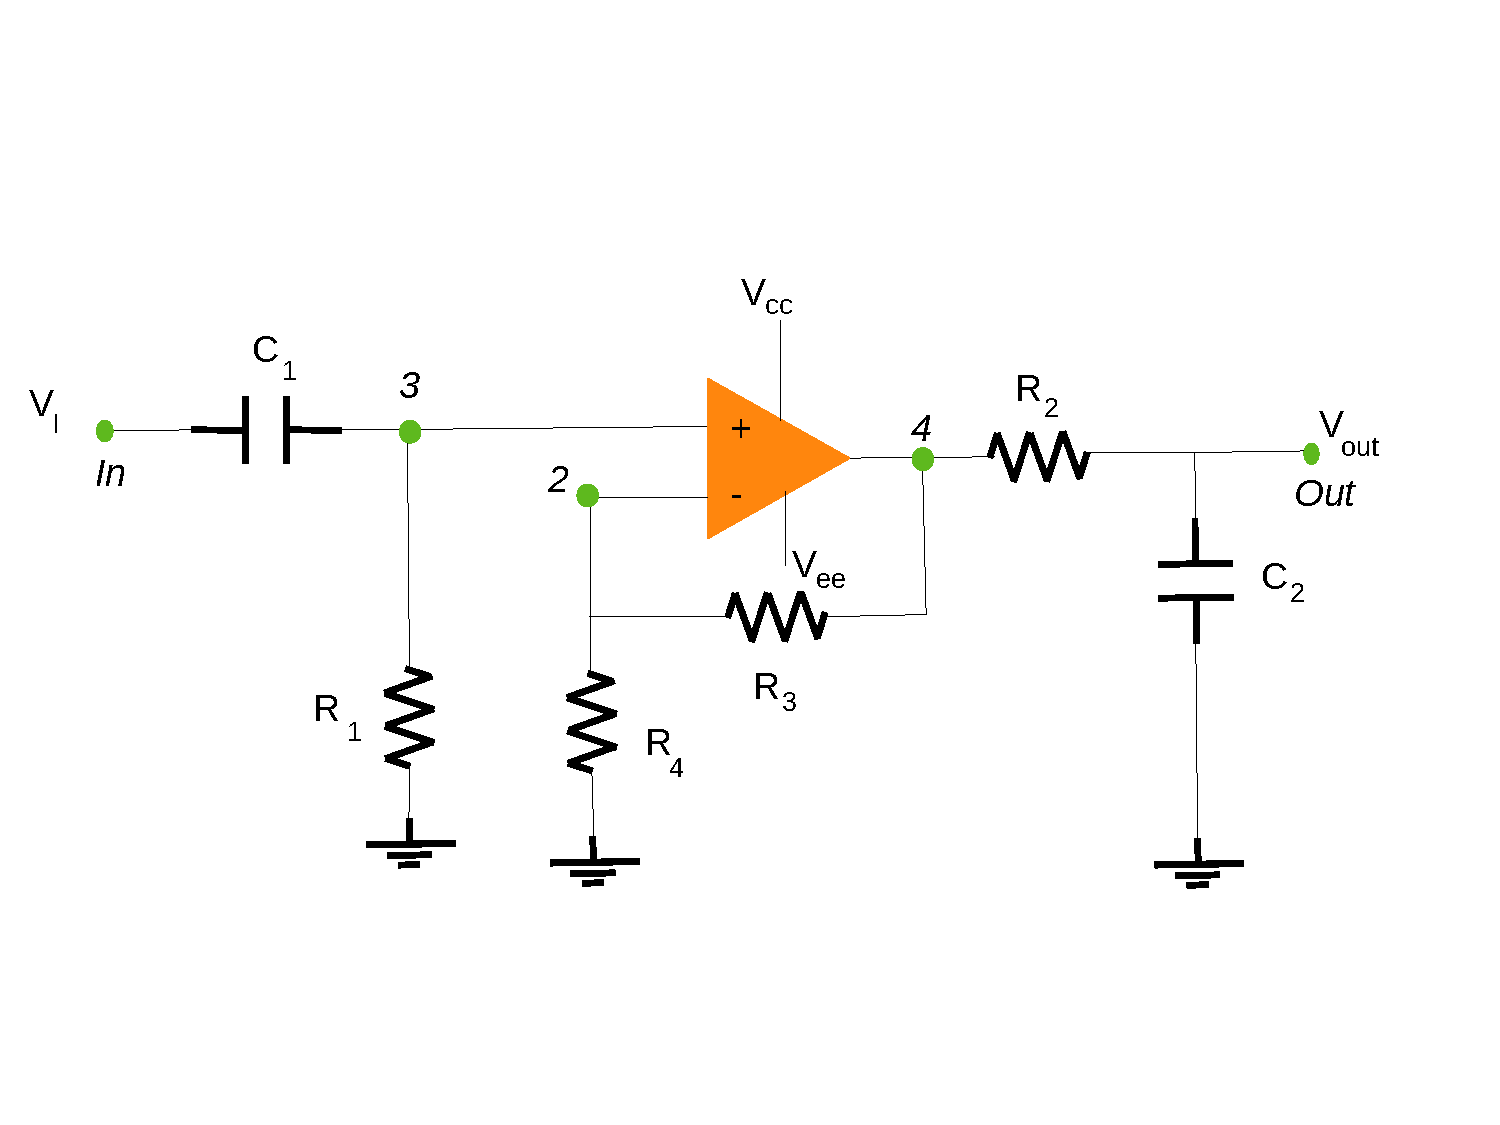
\includegraphics[width= 13cm]{circuito5.pdf} 
\caption{Main circuit}
\label{first}
\end{figure}

Note: The capacitor C2 represents two 220nF capacitors in series.

The constants values used are expressed in the following table.

%VALORES INTRO
\begin{table}[H] \centering
\begin{tabular}{|
>{\columncolor[HTML]{FFCC67}}l |c|}
\hline
\multicolumn{2}{|l|}{\cellcolor[HTML]{EABD8B}Name - Value} \\ \hline
C1 & 2.200000e-07 \\ \hline
C2 & 1.100000e-07 \\ \hline
R1 & 1.000000e+03 \\ \hline
R2 & 1.000000e+03 \\ \hline
R3 & 1.000000e+05 \\ \hline
R4 & 1.000000e+03 \\ \hline
Vcc & 1.000000e+01 \\ \hline

\end{tabular}
\caption{Initial Values}
\end{table}

In Section~\ref{sec:analysis}, a theoretical analysis of the circuit is
presented. In Section~\ref{sec:simulation}, the circuit is analysed by
simulation, and in Section~\ref{comparison} the results are compared to the theoretical results obtained in
Section~\ref{sec:analysis}. Next in Section~\ref{merit} we show the cost and merit atribuited to our circuit.
To finish, the conclusions of this study are outlined in Section~\ref{sec:conclusion}. \\




\section{Theoretical Analysis}
\label{sec:analysis}

In this section we will analyse theoretical our AC/DC converter circuit. \\
To do so, and because there were several things to be analysed, we divided the following subsections in the three different sectors that our circuit has and each one will be detailed separately.\\
Initially, we used a transformer to turn Vs=230V in a smaller value, being Vr=230/n, with n equal to 11, so that thew
rest of the circuit can aproximate it to 12 V that are requested. However, we want a DC voltage and not the initial AC voltage. In order
to achieve that, we are going to describe the three different sectors that are in the circuit that is shown in the Introdution.\\


\subsection{First sector: Bridge circuit}

The Bridge circuit is composed by the four diodes that are shown in the first figure.\\
The four diodes labelled $D_1$ to $D_4$ are arranged in "series pairs" with only two diodes conducting current during each half cycle. During the positive half cycle of the supple, diodes $D_1$ and $D_4$ conduct in series while diodes $D_2$ and $D_3$ are reverse biased and the current flows through the load.\\
Summarizing, these four diodes work as a full wave rectifier which means, they transform the AC current in an equal
amplitude unidirectional current, which corresponds to the module of the purple plot in figure 2. To compute all of that we had to take the absolute value of the transformed voltage $V_r$.

\subsection{Second sector: Envelope detector circuit (rectifier + capacitor)}

Then, we use a capacitor in order to reduce the magnitude of the voltage making it closer to a DC (orange plot).
In order to compute this, we discovered when are the diodes ON and OFF.\\
The equation that describes $t_{OFF}$ is:

\begin{equation} 
t_{OFF} = \frac{1}{2*w * arctan(1/(w*R_{1}*C)}
\label{eq2}
\end{equation}

It's 2 times the angular frequency just because we are using a full wave rectifier.

However to be more precise, we used the newton raphson method in the expressions obtained using the Kirchoff laws to determine both $t_{OFF}$ and $t_{ON}$.

Periodically, 

\begin{equation}
    \begin{cases}
      V_0=|V_r| & \text{$t<t_{OFF}$}\\
      V_0=|V_s*cos(w*t_{OFF})|*exp(-(t-t_{OFF})/(R1*c)) & \text{$t>t_{OFF}$}
    \end{cases}       
\end{equation}

due to the capacitor.\\
The ripple voltage is basically max($V_{0}$)- min($V_{0}$). \\


\begin{table}[H] \centering
\begin{tabular}{|
>{\columncolor[HTML]{FFCC67}}l |c|}
\hline
\multicolumn{2}{|l|}{\cellcolor[HTML]{EABD8B}Name - Value} \\ \hline
Ripple & 4.022790e-04\\ \hline
Average & 2.299980e+01\\ \hline

\end{tabular}
\caption{Ripple and average envelope values}
\end{table}

\subsection{Third sector: Voltage regulator circuit}

At last, in the third sector, a series of 22 diodes reduce the noise making the current an almost perfect DC.
By calculating the $v0_average$ from the second sector, we are able to see if the voltage difference between v5 and v0 is limited by
the maximum voltage that the diodes can handle. This only happens if the average is greater than that maximum.\\
Right now, we have the voltage due to the DC so we still need the voltage due to AC. It is possible to compute that in octave, calculating rD which is the resistance of each diode and also:

\begin{equation}
 ac_{v0} = num_{diodes}*rD/(num_{diodes}*rd+R2)*(Venvelope - average_{env})
\label{eq3}
\end{equation}

To finish, v0 = $ac_{v0}$ + $dc_{v0}$. 
The average must be approximately 12V.

\begin{table}[H] \centering
\begin{tabular}{|
>{\columncolor[HTML]{FFCC67}}l |c|}
\hline
\multicolumn{2}{|l|}{\cellcolor[HTML]{EABD8B}Name - Value} \\ \hline
Ripple & 1.915614e-05\\ \hline
Average & 1.200000e+01\\ \hline

\end{tabular}
\caption{Ripple and average regulator values}
\end{table}


\begin{figure}[H] 
\centering
\includegraphics[width = 8cm]{MainPlot.eps} 
\caption{Input voltage of the secondary circuit (v(2)), output Voltage of the Envelope Detector (v(4)), VoltageRegulator (v(5)), and v(5)-12}
\label{fig:first}
\end{figure}

\begin{figure}[H] 
\centering
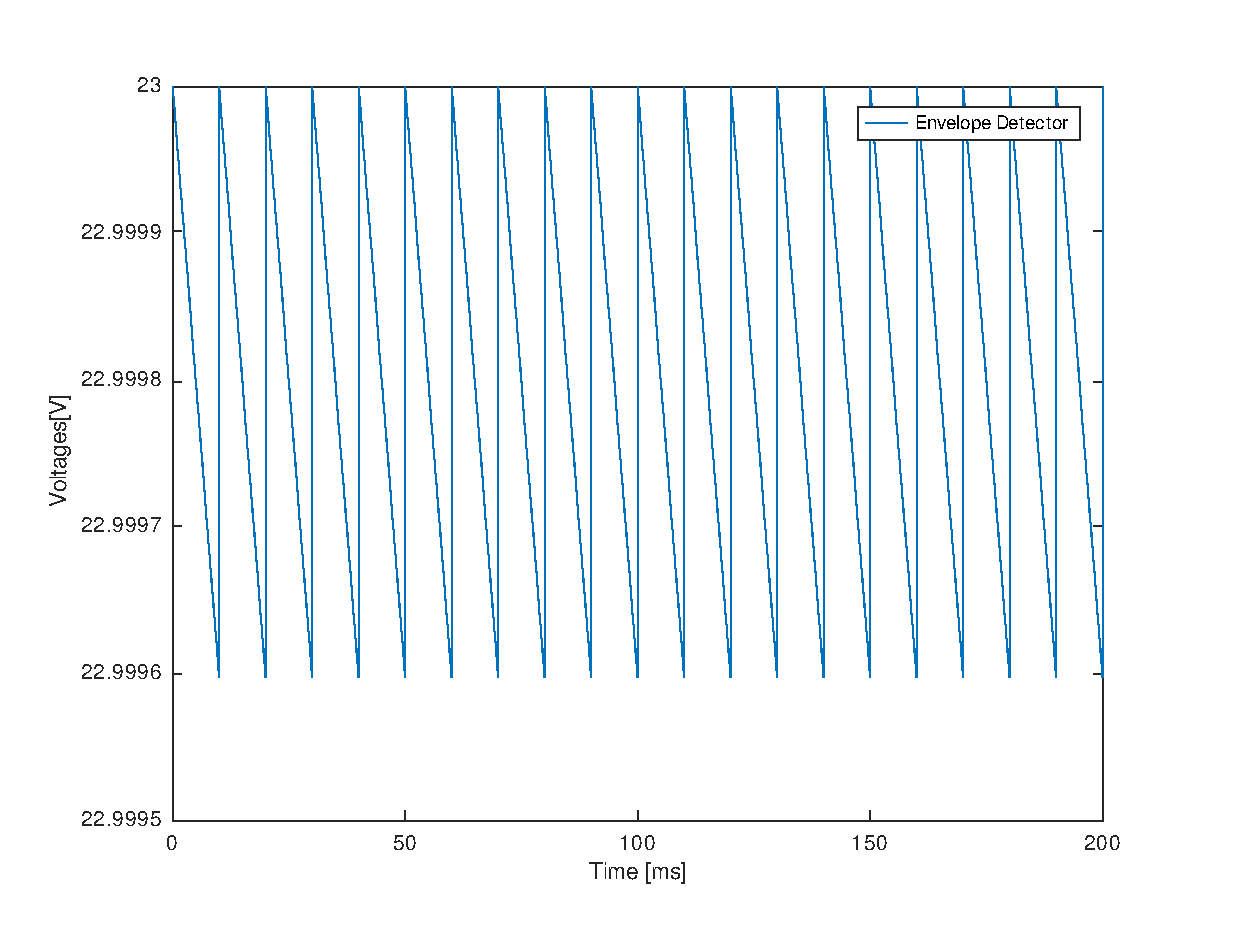
\includegraphics[width = 8cm]{EnvelopeDetector.eps} 
\caption{Output Voltage in Envelope Detector}
\label{fig:first}
\end{figure}

\begin{figure}[H] 
\centering
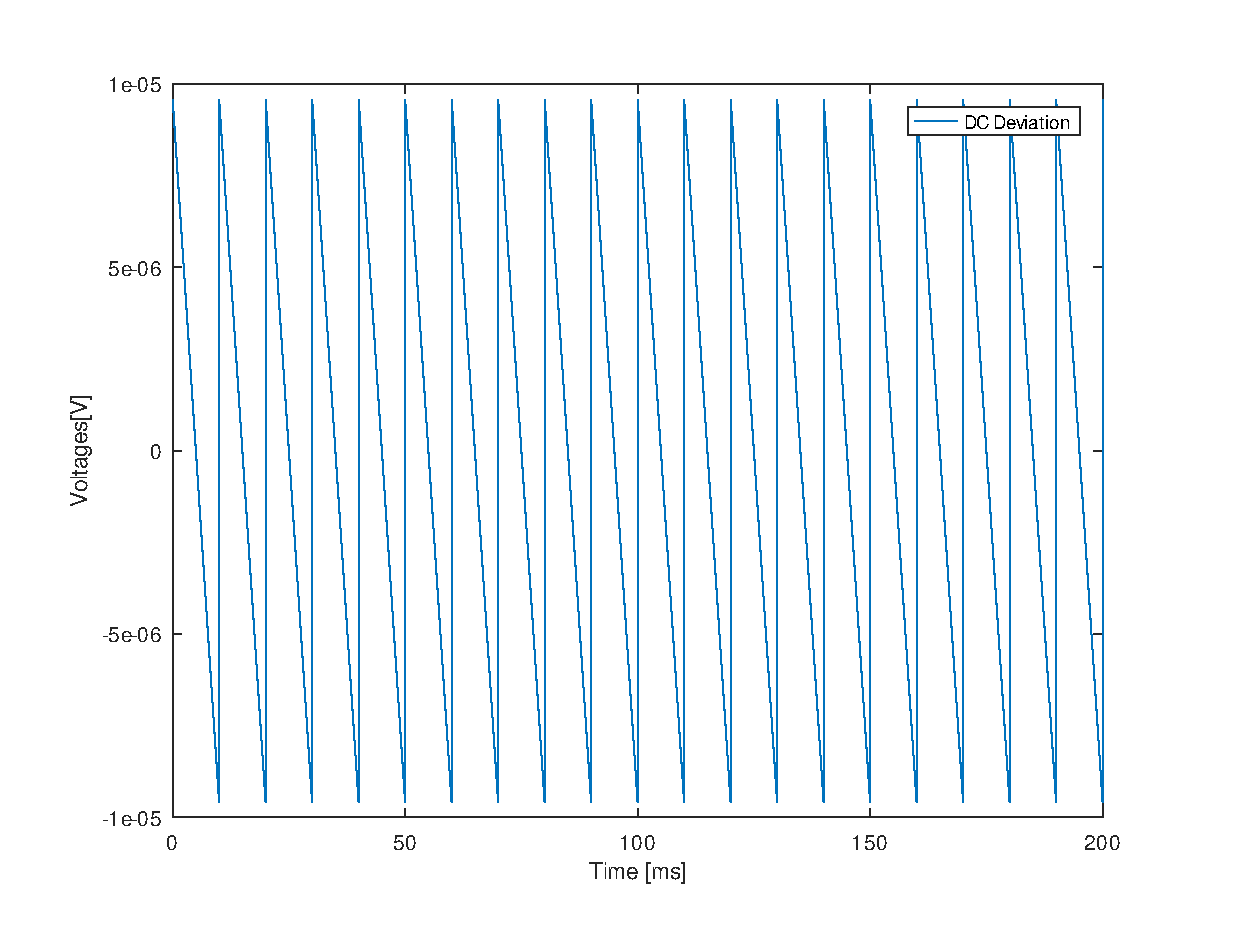
\includegraphics[width = 8cm]{DCDeviation.eps} 
\caption{Output DC Deviation}
\label{fig:first}
\end{figure}

\begin{figure}[H] 
\centering
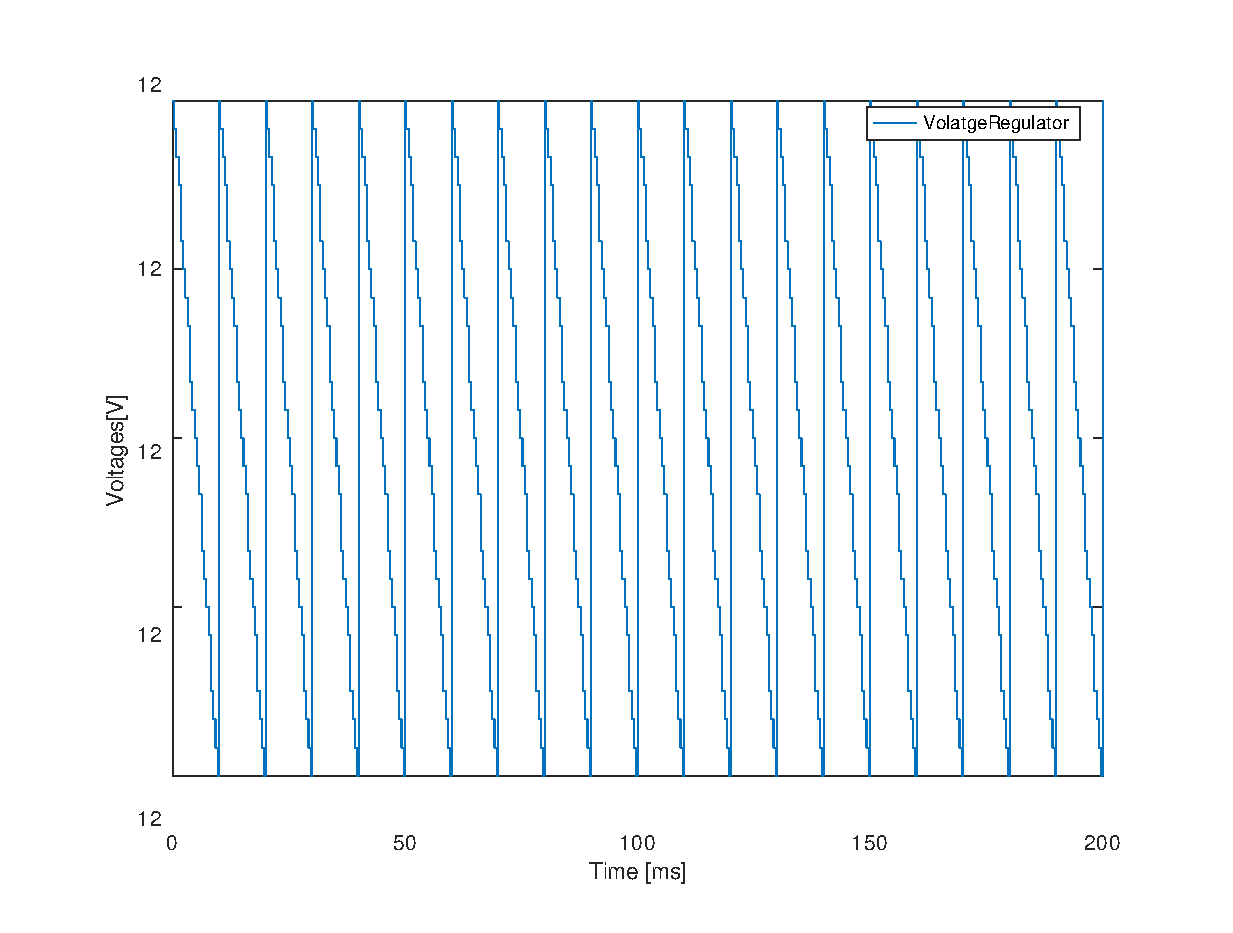
\includegraphics[width = 8cm]{VoltageRegulator.eps} 
\caption{Output Voltage}
\label{fig:first}
\end{figure}




\section{Simulation Analysis}
\label{sec:simulation}

\subsection{Operating point analysis for t$<$0}

In this section, an operating point analysis of the circuit (referência ao circuito) was conducted in order to calculate the voltage in all nodes and the current through the resistors for a t $<$ 0. To contextualize the values obtained using the tools in ngspice, it is necessary to state that, as node 0 is connected to ground, its nodal voltage does not appear on the table of results. It is important to note that an extra voltage source, Vaux, was added and therefore, another node was also added (node 9). This Vaux was intended to allow the measurement of the current Id which voltage source Vd depends on, since ngspice doesn't allow us to introduce Resistor R6's current in the computation. Vaux's voltage is equal to 0 V, since it is only an auxiliary component that doesn't interfere with the circuit (node's 7 voltage is equal to node's 9 voltage) and allowed us to obtain the current through it.

%Introduzir a primeira tabela dos valores das correntes e da tensão dos nós do spice e do octave lado a lado para comparar o erro
\begin{table}[h] 
\begin{minipage}{0.5\linewidth}
\centering
\begin{tabular}{|
>{\columncolor[HTML]{FFCC67}}l |c|}
\hline
\multicolumn{2}{|l|}{\cellcolor[HTML]{EABD8B}NgSpice - Voltages (V)} \\ \hline
@cb[i] & 0.000000e+00\\ \hline
@ce[i] & 0.000000e+00\\ \hline
@q1[ib] & 7.022567e-05\\ \hline
@q1[ic] & 1.404513e-02\\ \hline
@q1[ie] & -1.41154e-02\\ \hline
@q1[is] & 5.765392e-12\\ \hline
@rc[i] & 1.411536e-02\\ \hline
@re[i] & 1.411536e-02\\ \hline
@rf[i] & 7.022567e-05\\ \hline
@rs[i] & 0.000000e+00\\ \hline
v(1) & 0.000000e+00\\ \hline
v(2) & 0.000000e+00\\ \hline
base & 2.254108e+00\\ \hline
coll & 5.765392e+00\\ \hline
emit & 1.411536e+00\\ \hline
vcc & 1.000000e+01\\ \hline

\end{tabular}
\end{minipage}%
\begin{minipage}{0.5\linewidth}
\centering
\begin{tabular}{|
>{\columncolor[HTML]{FFCC67}}l |c|}
\hline
\multicolumn{2}{|l|}{\cellcolor[HTML]{EABD8B}Octave - Voltages (V)} \\ \hline
V1 & & 8.194795e+00 V\\ \hline
V2 & & 7.917828e+00 V\\ \hline
V3 & & 7.340169e+00 V\\ \hline
V4 & & 2.978754e+00 V\\ \hline
V5 & & 7.957540e+00 V\\ \hline
V6 & & 1.197664e+01 V\\ \hline
V7 & & 9.776608e-01 V\\ \hline
V8 & & 0.000000e+00 V\\ \hline

\end{tabular} 
\end{minipage}
\caption{Nodal Voltage Comparison}
\end{table}


\subsection{Calculus of $Req$ - Simulation}

Similarly to the last section, an operating point analysis to the circuit (referência ao circuito) was conducted, with the difference being that the voltage source $vs$ was turned off and the capacitor was replaced by the independent voltage source $Vx$ which corresponds to the value of $v(6)$-$v(8)$. This $Vx$ is equivalent to the voltage in the capacitor's terminals. 
The values of currents and nodal voltages were then put in a table, while the equivalent thevenin resistor was calculated by the following equation:

\begin{equation}
Req = (v(6)-v(8))/vxbranch,
\end{equation}
with $vxbranch$ corresponding to the current $Ix$ that flows through the $Vx$'s branch.

%Introduzir a primeira tabela dos valores das correntes e da tensão dos nós do spice e do octave lado a lado para comparar o erro
\begin{table}[h] 
\begin{minipage}{0.5\linewidth}
\centering
\begin{tabular}{|
>{\columncolor[HTML]{FFCC67}}l |c|}
\hline
\multicolumn{2}{|l|}{\cellcolor[HTML]{EABD8B}NgSpice - Voltages (V)} \\ \hline
@gb[i] & 0.000000e+00\\ \hline
@r1[i] & 0.000000e+00\\ \hline
@r2[i] & 0.000000e+00\\ \hline
@r3[i] & 0.000000e+00\\ \hline
@r4[i] & 0.000000e+00\\ \hline
@r5[i] & -1.63724e-02\\ \hline
@r6[i] & 0.000000e+00\\ \hline
@r7[i] & 0.000000e+00\\ \hline
v(1) & 0.000000e+00\\ \hline
v(2) & 0.000000e+00\\ \hline
v(3) & 0.000000e+00\\ \hline
v(5) & 0.000000e+00\\ \hline
v(6) & 5.000000e+01\\ \hline
v(7) & 0.000000e+00\\ \hline
v(8) & 0.000000e+00\\ \hline
v(9) & 0.000000e+00\\ \hline

\end{tabular}
\end{minipage}%
\begin{minipage}{0.5\linewidth}
\centering
\begin{tabular}{|
>{\columncolor[HTML]{FFCC67}}l |c|}
\hline
\multicolumn{2}{|l|}{\cellcolor[HTML]{EABD8B}Octave - Voltages (V)} \\ \hline
V1 & 0.000000e+00 V\\ \hline
V2 & -0.000000e+00 V\\ \hline
V3 & -0.000000e+00 V\\ \hline
V4 & -0.000000e+00 V\\ \hline
V5 & 0.000000e+00 V\\ \hline
V6 & 5.000000e+01 V\\ \hline
V7 & 0.000000e+00 V\\ \hline
V8 & -0.000000e+00 V\\ \hline

\end{tabular} 
\end{minipage}
\caption{Nodal Voltage Comparison}
\end{table}


\subsection{Transient Analysis for t $\geq$ (Natural Solution)}

In this section, a transient analysis was conducted in order to evaluate the natural response of the circuit, which means, the variation over time. Once that to calculate the natural response, the voltage source $vs$ is turned off, the circuit simulated was equal to the one in the previous question. From this, the voltage in the capacitor's over time (time interval considered was [0,20]ms) was calculated and plotted, using $Vx$ (calculated in the previous section) as the initial condition for the capacitor's voltage.

\begin{figure}[h] 
\centering
\begin{subfigure}{0.5\textwidth}
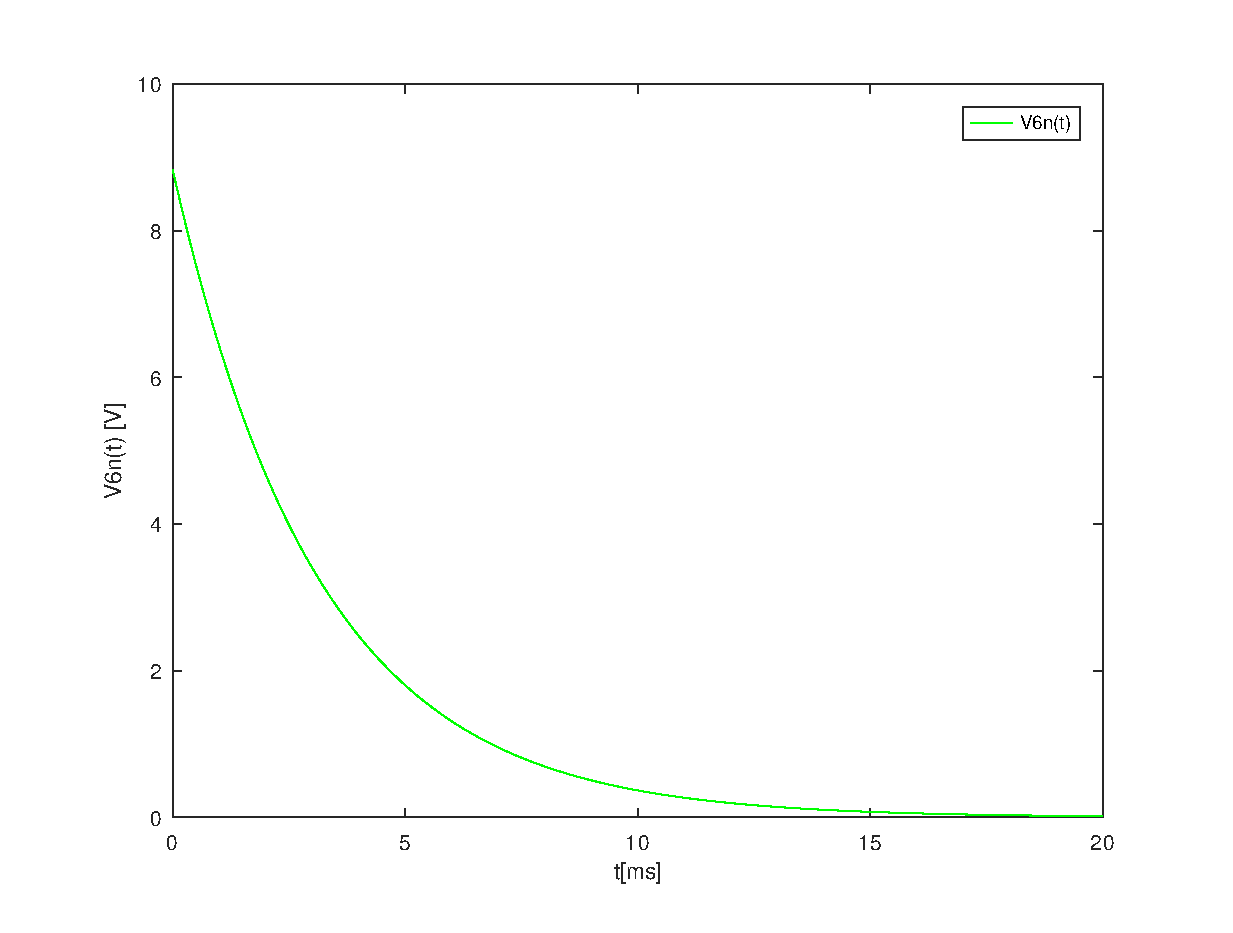
\includegraphics[width=\textwidth]{NaturalResponse.eps}
\caption{Natural Response (Octave)}
\label{fig:first}
\end{subfigure}
\begin{subfigure}{0.42\textwidth}
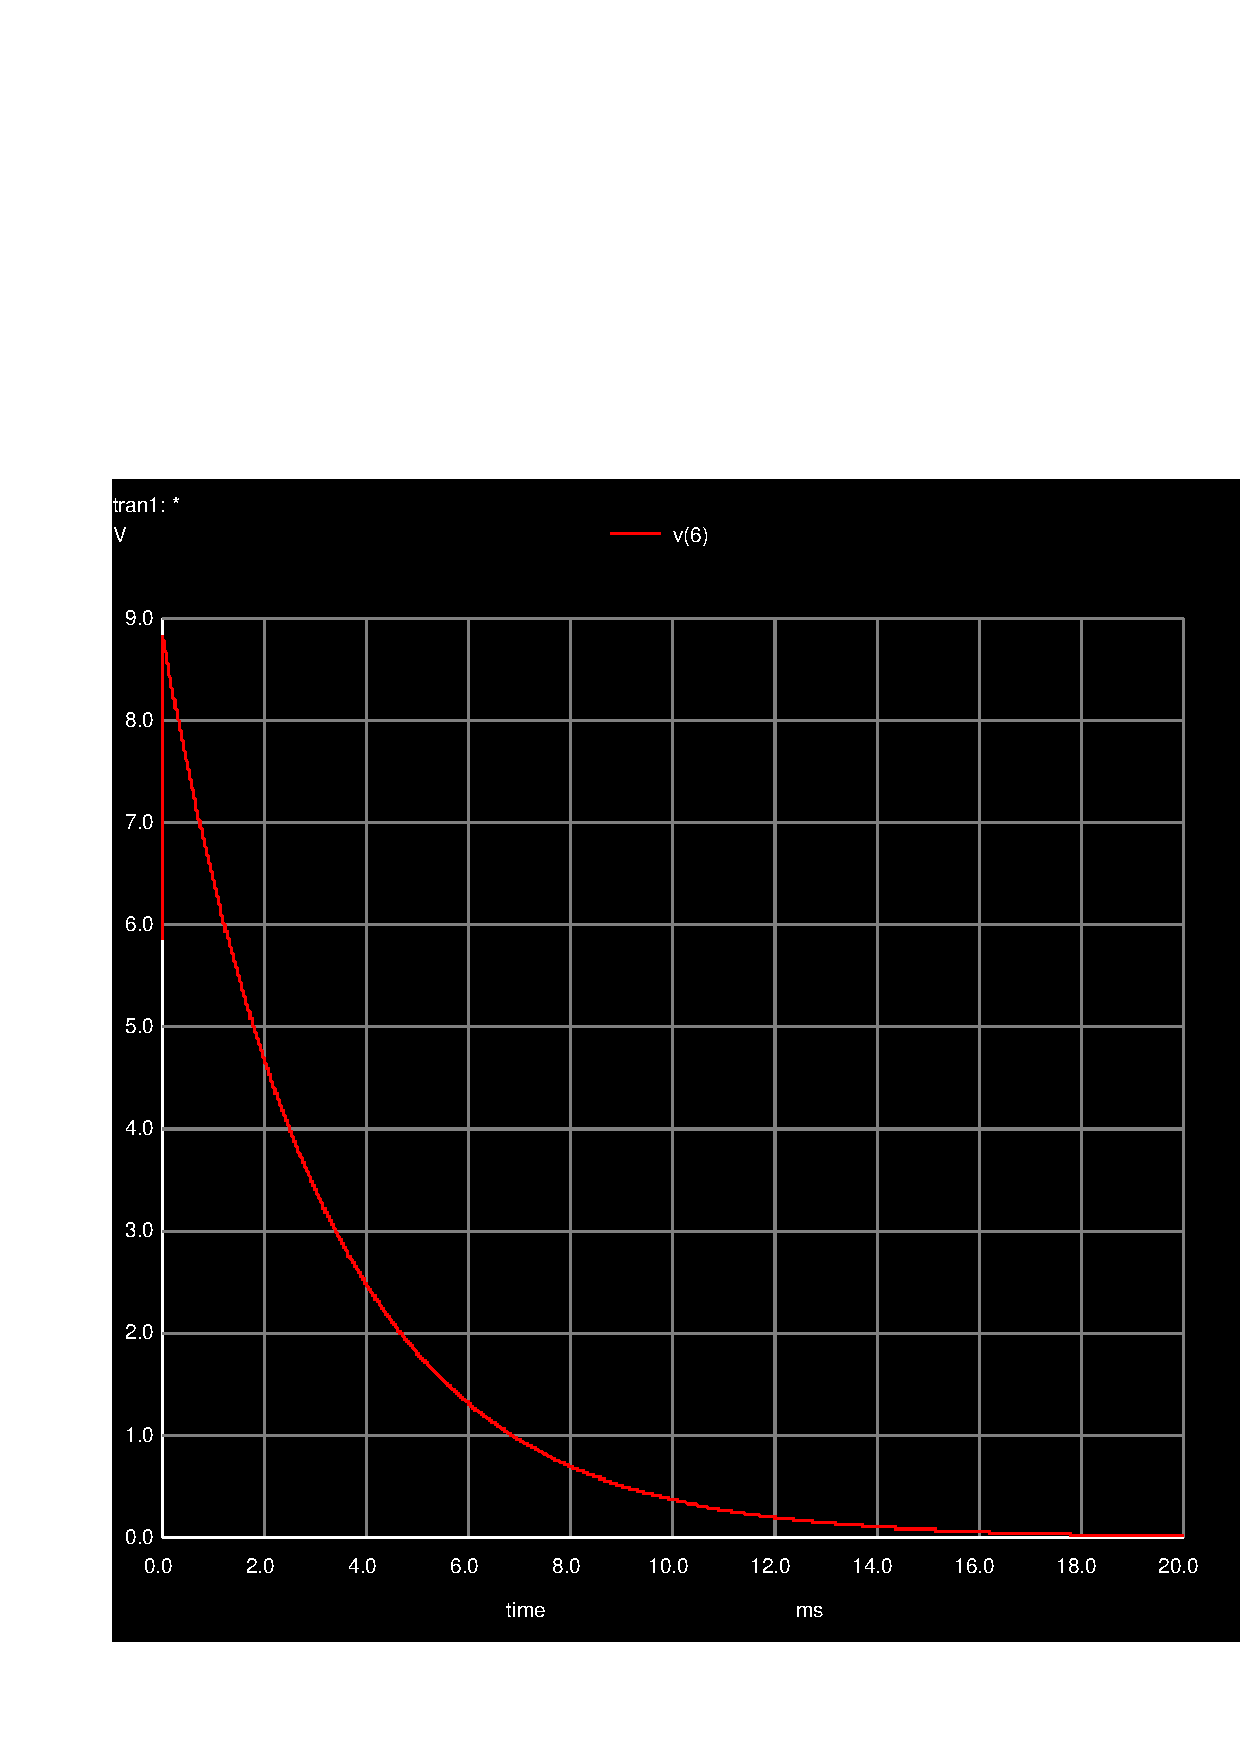
\includegraphics[width=\textwidth]{sim_3.pdf}
\caption{Natural Response (NGSpice)}
\label{fig:second}
\end{subfigure}
\end{figure}
 
 When observing the graph obtained from the simulation in Ngspice, we see that the capacitor's voltage overtime is a negative exponential matching the one obtained from the theorethical analysis in octave.
 
\pagebreak
 
\subsection{Operating Point Analysis for t $\geq$ (Natural and Forced Solution)}
In this section, as previously, a transient analysis was conducted in order to evaluate the natural and forced response of the circuit. In order to achieve this, the procedure adopted was the same as the one in the previous step, but with the voltage souce $vs(t)$ consisting of a sinusoidal wave sen(2*$\pi$*f).  

\begin{figure}[h] 
\centering
\begin{subfigure}{0.5\textwidth}
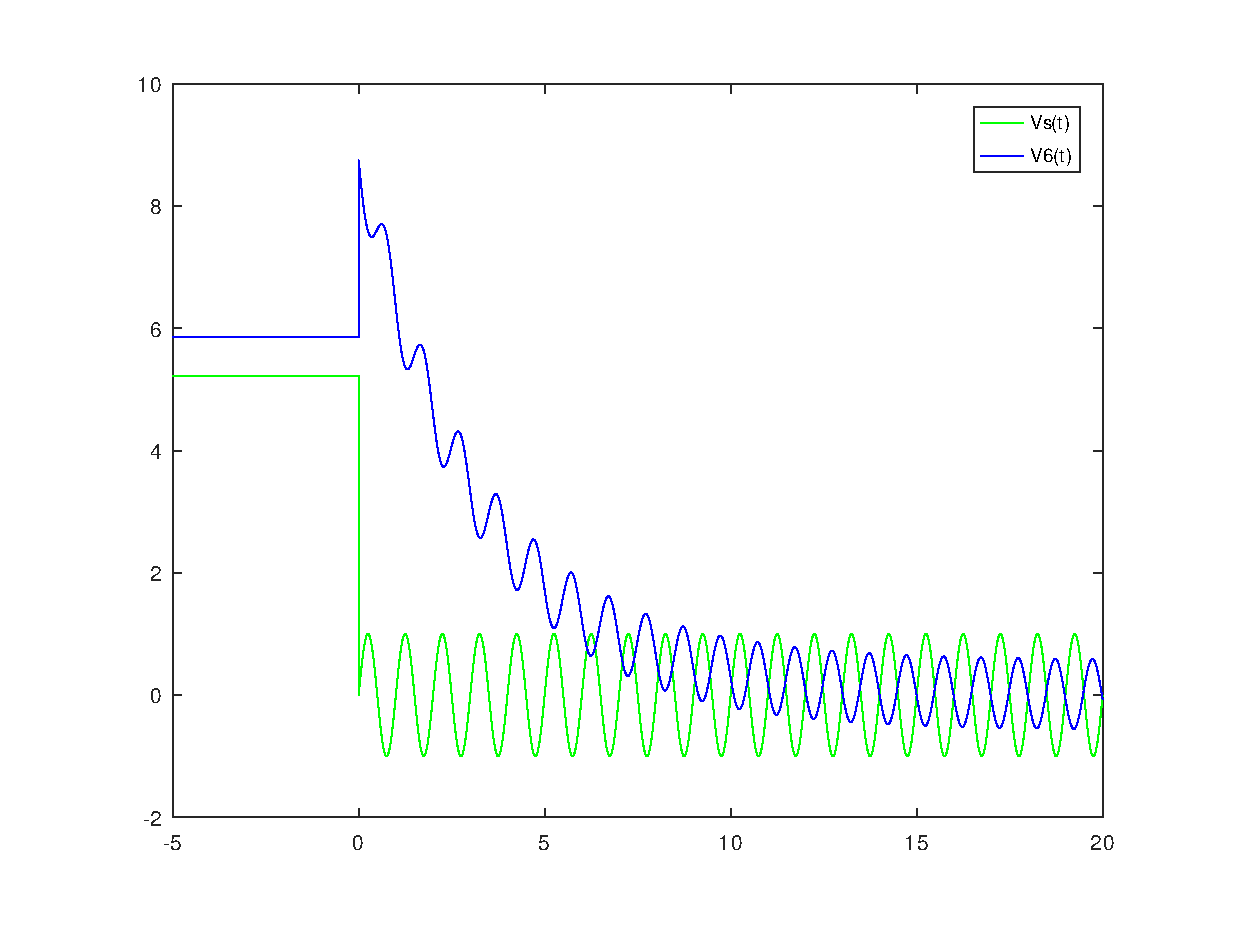
\includegraphics[width=\textwidth]{Solution.eps}
\caption{Natural and forced response (Octave)}
\label{fig:first}
\end{subfigure}
\begin{subfigure}{0.42\textwidth}
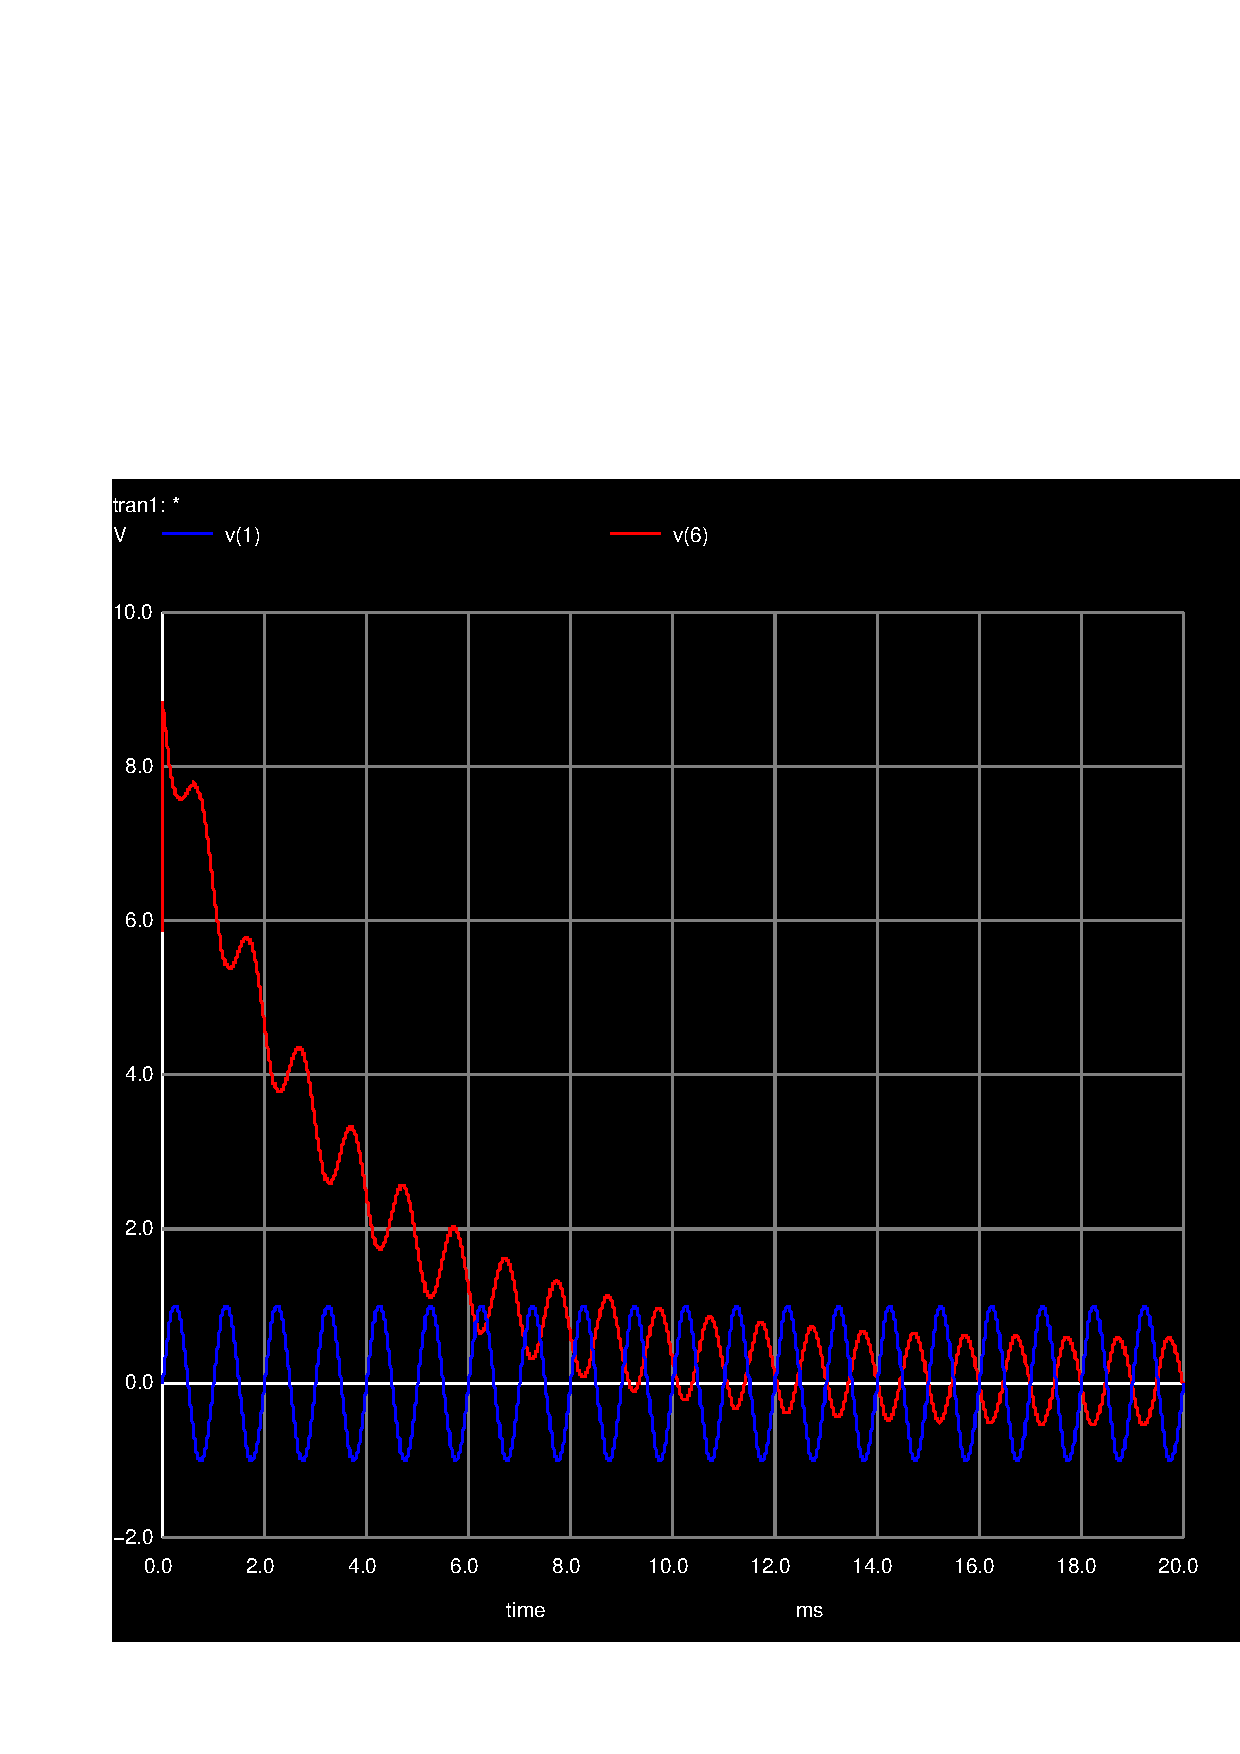
\includegraphics[width=\textwidth]{sim4.pdf}
\caption{Natural and forced response}
\label{fig:second}
\end{subfigure}
\end{figure}

When observing the graph obtained from the simulation  Ngspice, it is possible to conclude that, over the period of time considered, the voltage in the capacitor tends
to diminuish until its phase differs $\pi$ from the phase of the voltage source, such as in the graph obtained from the theorethical analysis in octave.

\subsection{Frequency Responses}

In this part of the assignment, an AC (Alternating Current) Analysis was conducted, in order to match the goal mentioned above. This type of analysis allows to study the frequency response of the circuit. For this, there is no frequency variation (steady-state analysis). After comparing the graphics showed below, it is clear to admit that the results in ngspice and octave match. Any minor difference may be explained by aproximation errors.

\subsubsection{Frequency Responses - Amplitude}

\begin{figure}[H] 
\centering
\begin{subfigure}{0.5\textwidth}
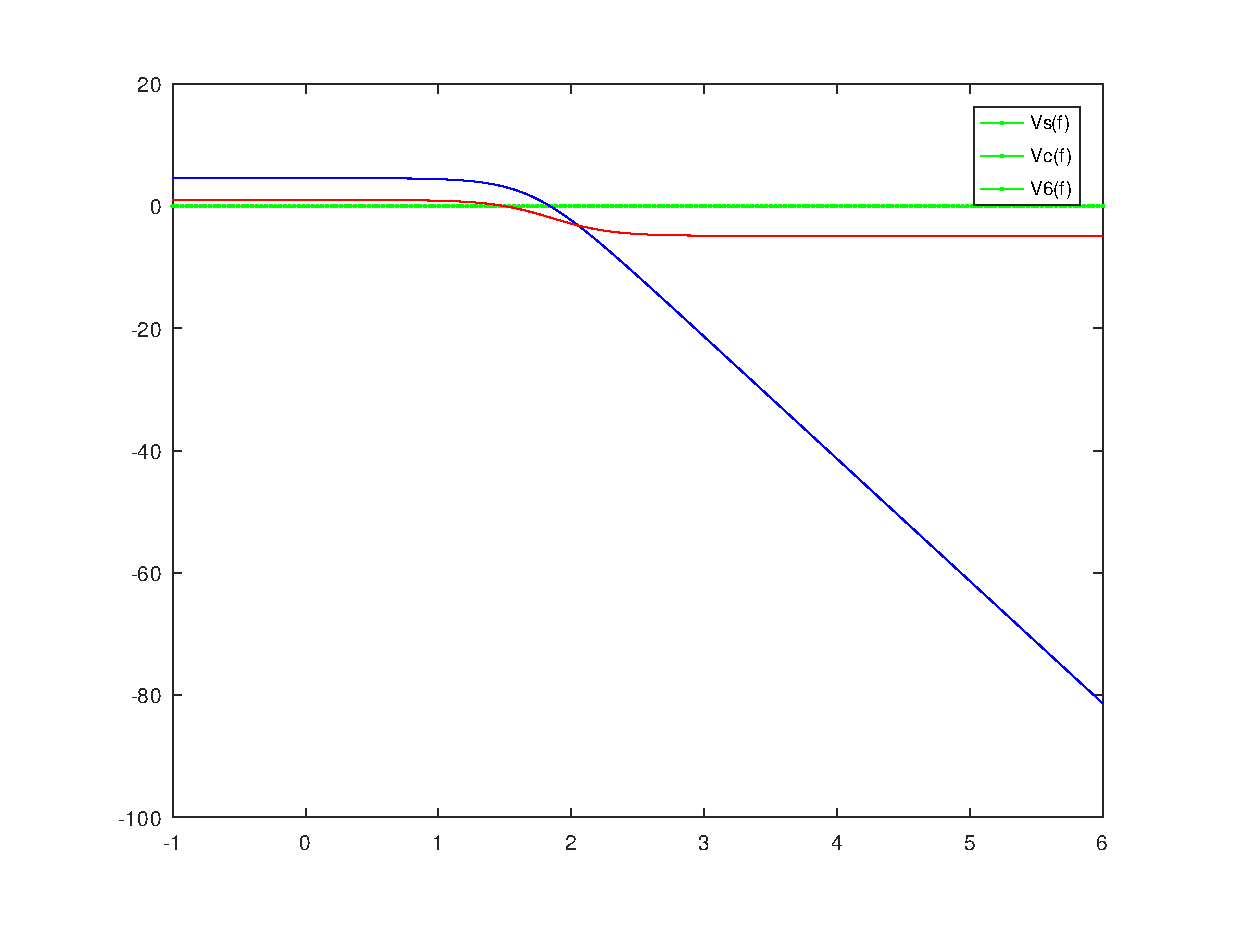
\includegraphics[width=\textwidth]{Amplitude.eps}
\caption{Amplitude (Octave)}
\label{fig:first}
\end{subfigure}
\begin{subfigure}{0.42\textwidth}
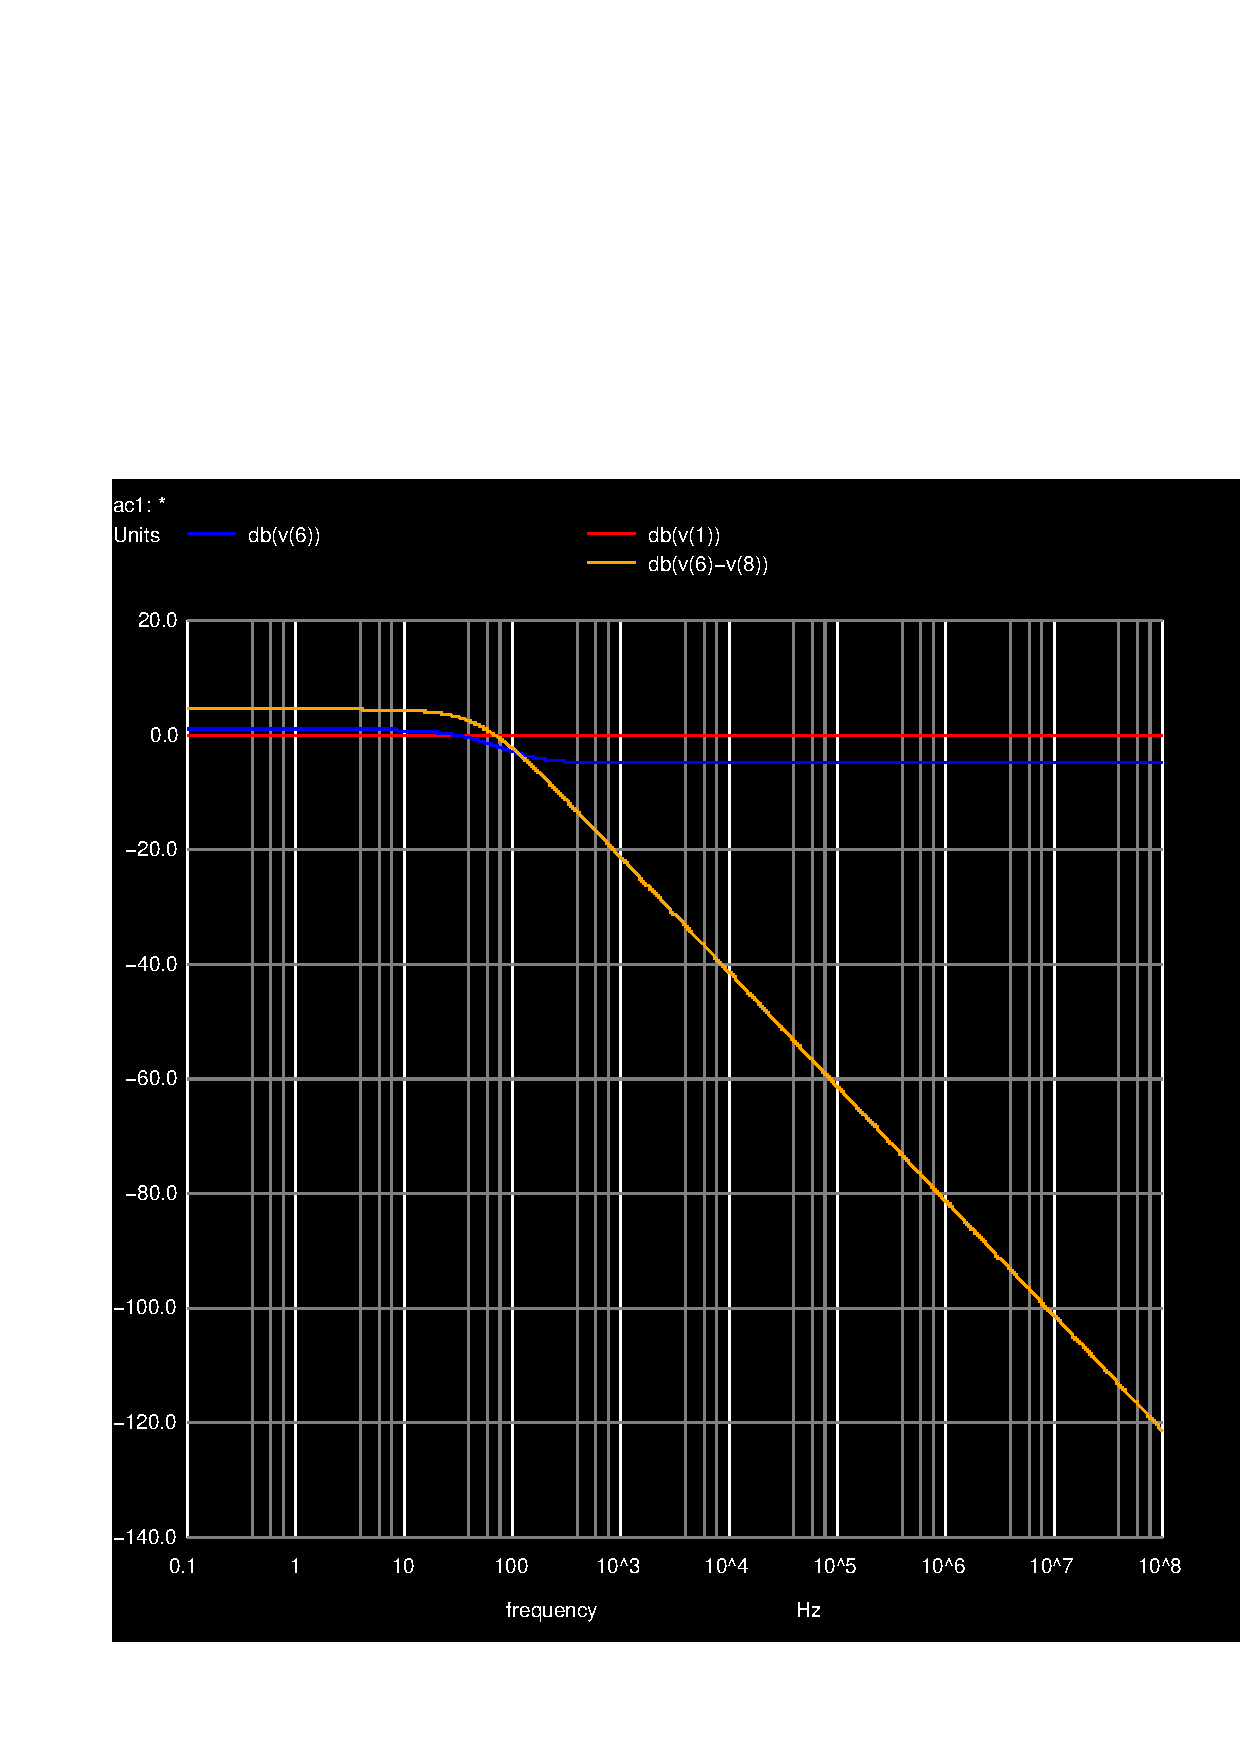
\includegraphics[width=\textwidth]{sim5_db.pdf}
\caption{Amplitude (NgSpice)}
\label{fig:second}
\end{subfigure}
\end{figure}

As expected, the results obtained from the ngspice simulation and the theorethical analysis in octave match.

\subsubsection{Frequency Responses - Phase}

\begin{figure}[H] 
\centering
\begin{subfigure}{0.5\textwidth}
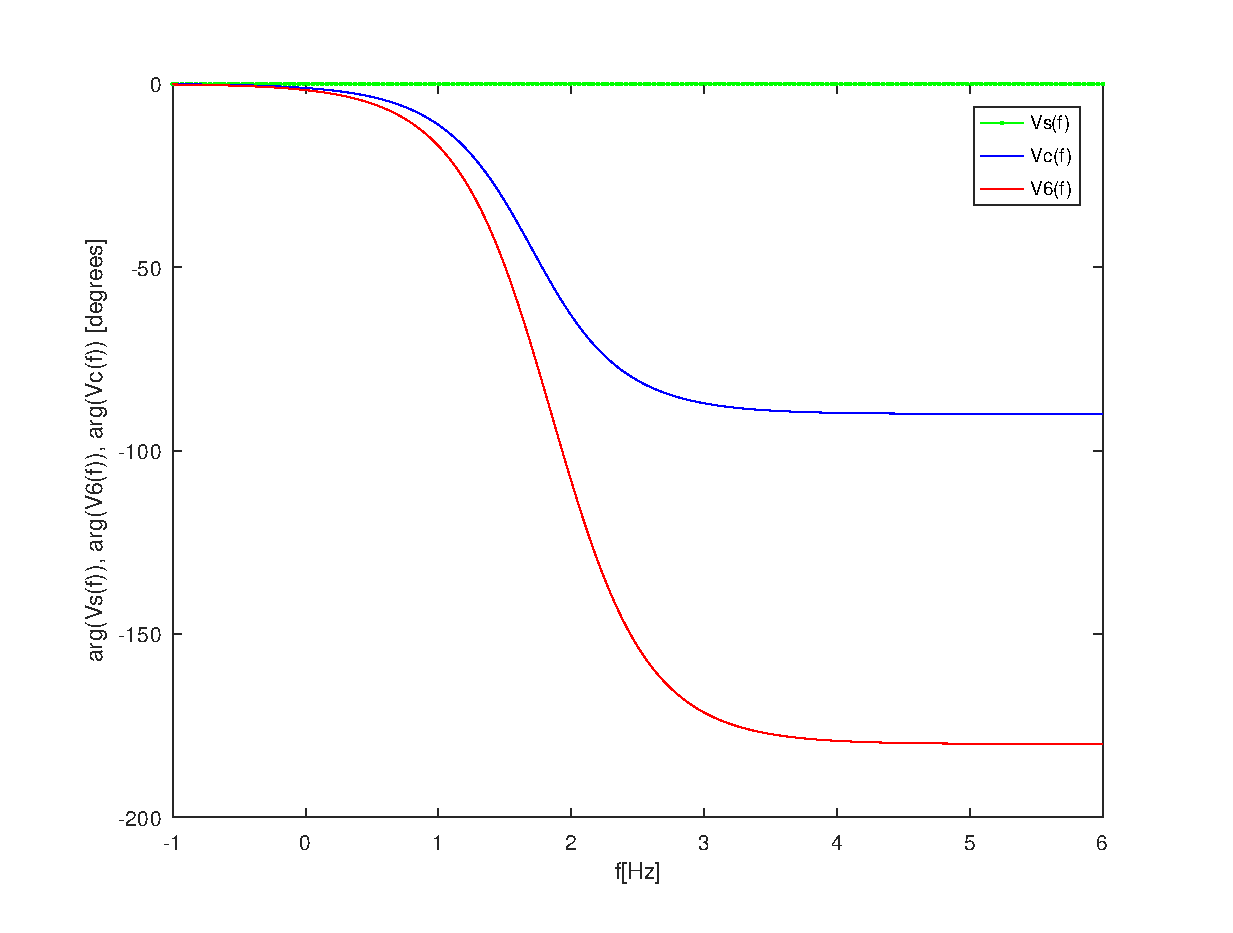
\includegraphics[width=8cm]{Arguments.eps}
\caption{Arguments (Octave)}
\label{fig:first}
\end{subfigure}
\begin{subfigure}{0.42\textwidth}
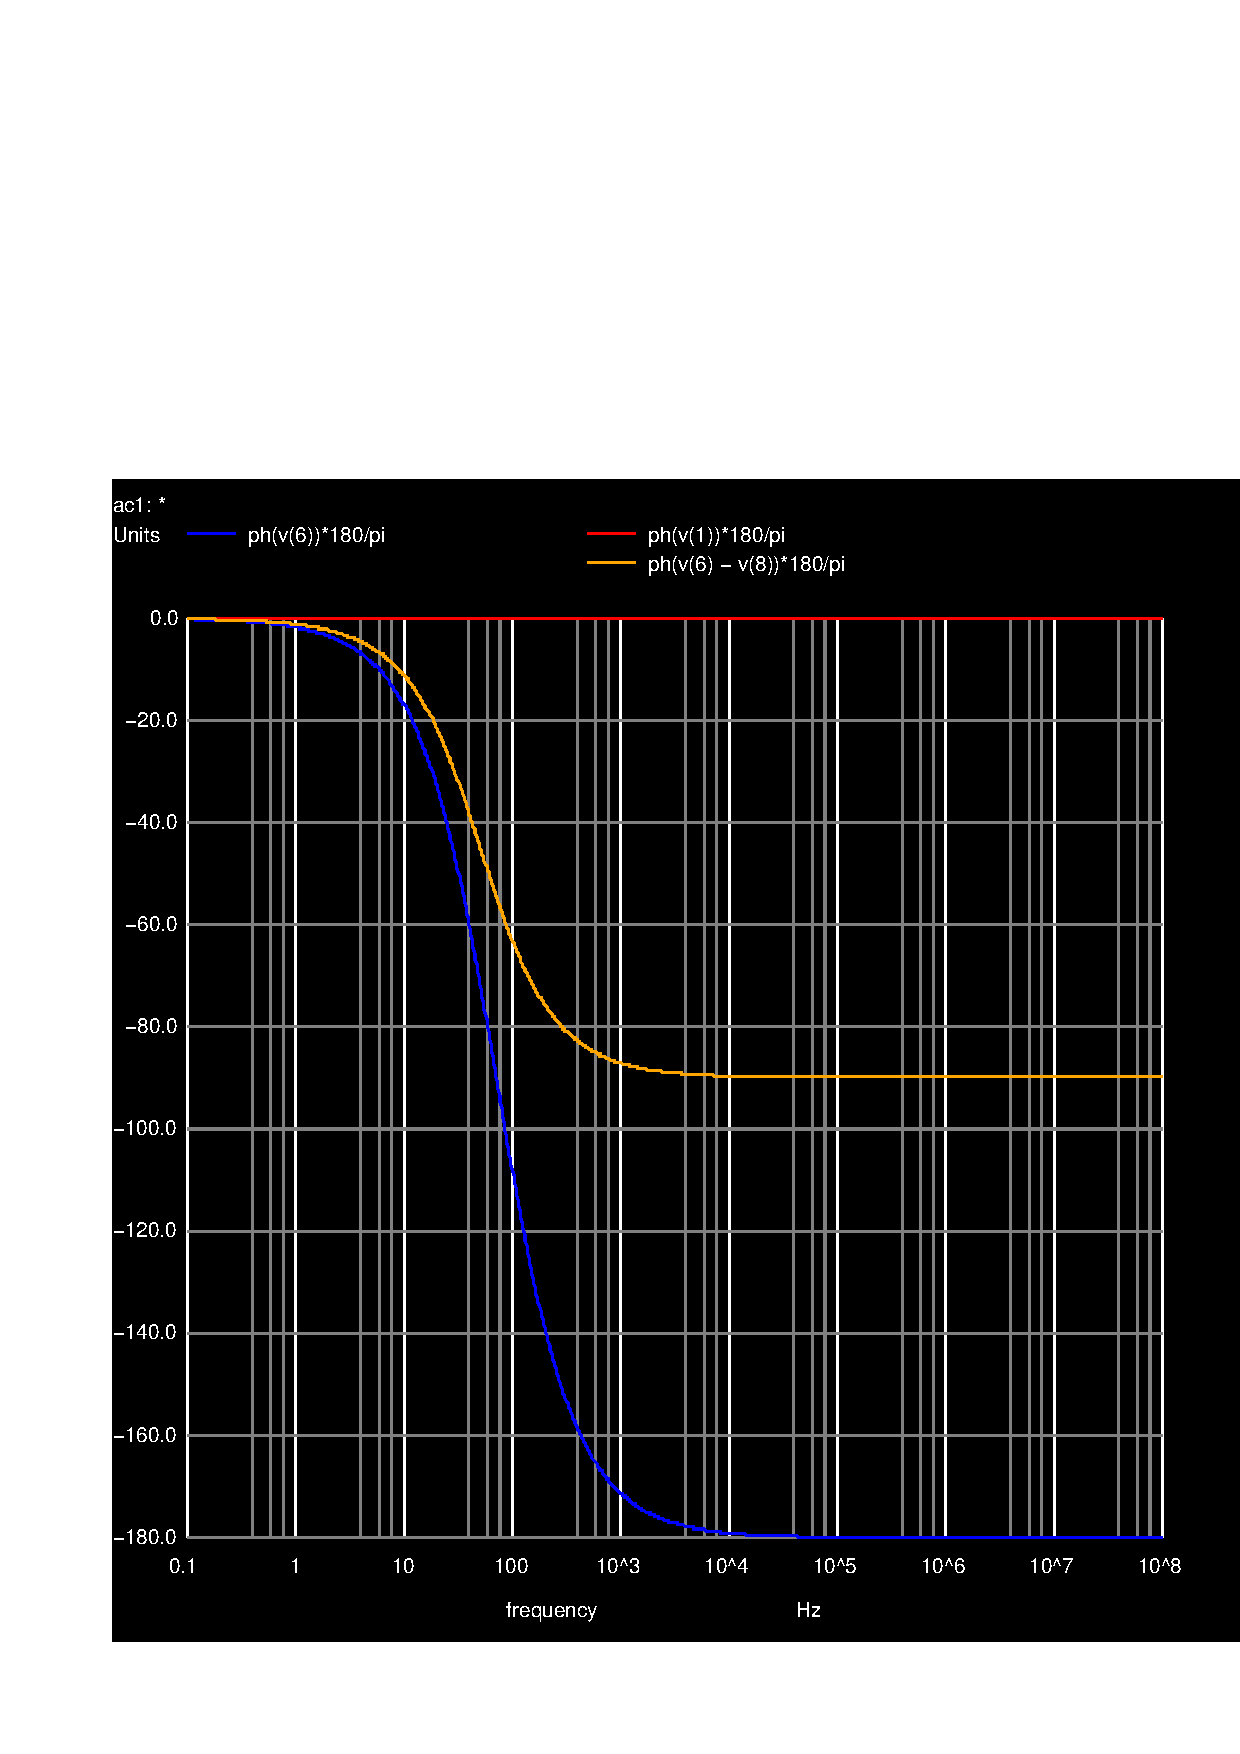
\includegraphics[width=8cm]{sim5_ph.pdf}
\caption{Arguments (NgSpice)}
\label{fig:second}
\end{subfigure}
\end{figure}

As expected, the results obtained from the ngspice simulation and the theorethical analysis in octave match.



\section{Conclusion}
\label{sec:conclusion}

In this laboratory assignment, the objective of analysing the circuit especified in the introduction has been
achieved. All analyses have been performed both theoretically using the Octave maths tool and by circuit simulation using the
Ngspice tool. When comparing these last two we conclude that there aren't any disparity between the results and therefore no errors associated.\\
So we conclude that the methods utilized to analyse the circuit in question can be validated.


%\cleardoublepage

% ----------------------------------------------------------------------
%  Bibliography
% ----------------------------------------------------------------------
%\addcontentsline{toc}{section}{\bibname}
%\bibliographystyle{abbrvunsrtnat} % <<<<< SELECT IF USING REFERENCES BY NUMBER (CITATION ORDER)
%\bibliography{../../../BIBfile.bib}

% ----------------------------------------------------------------------
\end{document}
% ----------------------------------------------------------------------
